\ifthenelse{\equal{\doclanguage}{Italian}}
{\chapter{Implementation}}
{\chapter{Implementazione}}
\label{sec:implementation}

% NON SO SE TRASFORMARLE IN SEZIONI O LASCIARLE SUB
\vspace{-10pt}
\section{Configurazione dell'Ambiente e del Cluster Neo4j}
% Qui descrivi: il setup delle macchine/WSL2, la topologia del cluster distribuito, la configurazione della memoria e l'installazione delle librerie (es. PyTorch Geometric, driver Neo4j).

L'infrastruttura sperimentale è distribuita su quattro macchine virtuali Microsoft Azure, ciascuna equipaggiata con Windows 10 all'interno del quale è stato installato il \textit{Windows Subsystem Linux} V2 con Ubuntu 22.04 LTS. Le macchine hanno 8 vcore e 32 GB di RAM. La scelta di WSL2 come layer di virtualizzazione ha permesso di eseguire container Docker nativi su Linux mantenendo performance comparabili a un ambiente Linux nativo e con la possibilità di configurare il sistema in modo più aperto. Neo4j Enterprise 2026.04.0 gira all'interno di container Docker su WSL2, orchestrati tramite un file \texttt{docker-compose.yml} condiviso tra tutti i nodi del cluster, che definisce i servizi, le variabili d'ambiente e i volumi persistenti per ciascuna istanza.

La topologia adottata prevede un nodo primary e tre nodi secondary. Il primary gestisce tutte le operazioni di scrittura e coordina il consenso distribuito tramite il protocollo Raft, mentre il router integrato di Neo4j gestisce il bilanciamento del carico delle letture tra le secondary. I secondary sono dedicati esclusivamente alla lettura distribuita e al calcolo analitico, senza partecipare alle operazioni di scrittura. La scelta di quattro nodi totali non è motivata dalla fault tolerance ma dall'obiettivo di misurare l'impatto della scalabilità orizzontale sui tempi di estrazione dei dati e di valutare il comportamento del routing layer in presenza di molteplici repliche.

Ogni container Neo4j è stato configurato con limiti di memoria espliciti, bilanciando le esigenze del garbage collector della Java Virtual Machine e la velocità di accesso ai dati tramite page cache:

\begin{lstlisting}[caption={Configurazione memoria Neo4j (neo4j.conf)}]
server.memory.heap.initial_size=8G
server.memory.heap.max_size=8G
server.memory.pagecache.size=6G
\end{lstlisting}

I limiti a livello Docker sono stati impostati a 20 GB per container, con 6 GB riservati al sistema operativo WSL2. L'heap da 8 GB è dedicato al garbage collector della JVM, mentre i 6 GB di page cache accelerano le letture mantenendo in memoria le porzioni del grafo più frequentemente accedute. Questa suddivisione è stata calibrata per bilanciare il throughput delle query, garantendo al contempo che il garbage collector non introduca pause significative durante le operazioni di lettura intensiva sul sottografo.

L'adozione di WSL2 ha introdotto una complicazione tecnica rilevante: l'indirizzo IP interno assegnato da WSL2 cambia ad ogni riavvio del sistema operativo Windows, rendendo instabili le regole di port-forwarding configurate staticamente. Il problema è stato risolto tramite uno script PowerShell automatizzato, eseguito all'avvio di ogni macchina con privilegi di amministratore, che interroga WSL2 per ottenere l'IP corrente e aggiorna dinamicamente le regole di port-forwarding tramite \texttt{netsh} sulle porte necessarie alla comunicazione intra-cluster (6000 per le transazioni, 7000 per il protocollo Raft, 7687 per il protocollo Bolt, 22 per l'SSH), garantendo che il cluster mantenga la connettività intra-cluster anche dopo riavvii non pianificati.

L'intera gestione del cluster è automatizzata tramite Ansible, eseguito dalla primary via SSH verso le secondary. I playbook principali sono \texttt{deploy.yml} per distribuire le configurazioni e avviare i container, \texttt{stop.yml} per fermarli in modo ordinato, \texttt{reset.yml} per un reset completo e \texttt{setup.yml} per la creazione della struttura di cartelle. Le variabili specifiche di ciascun nodo, come nome, ruolo e indirizzo IP, sono isolate in un file \texttt{.env} generato da Ansible tramite un template Jinja2, garantendo che la configurazione sia riproducibile e centralizzata senza interventi manuali su ogni macchina. 

L'uso di Ansible consente inoltre di eseguire il benchmark nelle diverse configurazioni (1, 2 o 4 nodi) in modo sistematico, variando il parametro \texttt{nodes} al momento dell'esecuzione del playbook. Questo approccio garantisce che ogni configurazione venga testata nelle stesse condizioni operative, eliminando possibili fonti di variabilità legate a interventi manuali sul cluster. La riproducibilità delle misurazioni è ulteriormente assicurata dall'esecuzione di un set di query di riscaldamento prima di ogni benchmark, che porta il database a regime termico.

La gestione delle dipendenze Python è affidata a \textbf{uv}, un package manager ad alte prestazioni che parallelizza il download e la risoluzione delle dipendenze, garantendo riproducibilità tramite un file \texttt{pyproject.toml}. Rispetto ai tradizionali gestori di pacchetti, uv riduce significativamente i tempi di installazione, un aspetto non trascurabile quando si lavora con ambienti di sviluppo containerizzati e si devono replicare frequentemente gli esperimenti. Le librerie necessarie alla pipeline sono installate con un singolo comando:

\begin{lstlisting}[language=bash, caption={Installazione delle librerie della pipeline sperimentale}]
uv add torch torch_geometric neo4j \
       pandas numpy scikit-learn
\end{lstlisting}

Gli script Python vengono eseguiti tramite \texttt{uv run}, che attiva automaticamente l'ambiente virtuale isolato prima dell'esecuzione, eliminando conflitti tra dipendenze di progetti diversi. Questo approccio garantisce che l'ambiente di esecuzione sia sempre coerente con le specifiche dichiarate, semplificando la collaborazione e la condivisione del codice.

\section{Acquisizione e Ingestion del Dataset}
% Qui descrivi: la provenienza del dataset (es. Zenodo), il formato originale (dump Neo4j), e il processo di caricamento (load) e distribuzione (seeding) sui nodi del cluster.
Il dataset è distribuito pubblicamente tramite Zenodo \cite{pharmebinet_zenodo} in formato dump nativo Neo4j, ovvero un archivio binario che rappresenta lo stato completo del database a grafo e può essere caricato direttamente tramite il tool \texttt{neo4j-admin} senza richiedere alcuna fase di conversione o pre-processing. 

Questo formato garantisce che il caricamento preservi integralmente la struttura del grafo, inclusi gli indici e i vincoli di integrità definiti nel database originale. Il file dump è stato scaricato sulla macchina primary e copiato nella cartella \texttt{data/raw/} del progetto.

Il caricamento è avvenuto tramite un container Docker effimero della stessa immagine Neo4j, che accede direttamente al layer di storage bypassando il motore transazionale, la modalità più efficiente per l'importazione massiva di dati. Questa strategia evita l'overhead delle transazioni e riduce il tempo complessivo di caricamento, consentendo di importare il grafo da 50 GB in tempi compatibili con lo sviluppo sperimentale. Al termine del caricamento, il container viene automaticamente rimosso, lasciando il database pronto per la successiva fase di configurazione del cluster.

\begin{lstlisting}[language=bash, caption={Caricamento del dump PharMeBiNet V3}]
docker run --rm -it \
  -e NEO4J_ACCEPT_LICENSE_AGREEMENT=yes \
  -v $(pwd)/cluster/data:/data \
  -v $(pwd)/data/raw:/backups \
  neo4j:2026.04.0-enterprise \
  neo4j-admin database load pharmebinet \
    --from-path=/backups/ \
    --overwrite-destination=true
\end{lstlisting}

Al termine del caricamento sulla primary, il database è stato distribuito automaticamente sulle secondary tramite il meccanismo di seeding nativo di Neo4j Cluster. La distribuzione avviene tramite una query Cypher che istruisce il cluster a replicare i dati esistenti a partire dal nodo sorgente specificato:

\begin{lstlisting}[language=Cypher, caption={Creazione del database distribuito con seeding}]
CREATE DATABASE pharmebinet
  TOPOLOGY 1 PRIMARY 3 SECONDARY
  OPTIONS {
    existingData: 'use',
    existingDataSeedServer: '<SERVER_ID_PRIMARY>'};
\end{lstlisting}

Il processo di replica di circa 50 GB ha richiesto diversi minuti, al termine dei quali tutti e quattro i nodi risultavano \texttt{online} per il database \texttt{pharmebinet}, pronti a servire sia operazioni di scrittura sul primary sia di lettura sui secondary. Una volta completata la replica, è stata verificata la consistenza del grafo attraverso query di conteggio sui nodi e sulle relazioni, confermando che il dataset era stato distribuito correttamente senza perdita di informazioni.

\section{Data Preprocessing ed Estrazione del Sottografo}
% Qui descrivi: l'analisi esplorativa preliminare (EDA) sul grafo completo e le query Cypher utilizzate per isolare ed estrarre le entità e le relazioni di interesse (Chemical e Disease).

Prima di procedere con la sperimentazione, il grafo è stato sottoposto a un'analisi esplorativa sistematica tramite query Cypher eseguite su Neo4j Browser, con l'obiettivo di caratterizzarne la struttura topologica e di identificare il sottografo tematico più adatto al task di link prediction.

\begin{lstlisting}[language=Cypher, caption={Query EDA su PharMeBiNet}]
CALL apoc.meta.stats()
YIELD labels, relTypesCount, nodeCount, relCount
RETURN labels, relTypesCount, nodeCount, relCount
\end{lstlisting}

I risultati confermano la forte eterogeneità del dataset. I nodi dominanti per cardinalità sono le varianti genomiche (\texttt{Variant}, \texttt{GeneVariant}, \texttt{SNV}, circa 3,8 milioni ciascuno), seguiti da modificazioni post-traduzionali (\texttt{PTS}, 782 mila), composti chimici (\texttt{Chemical}, 594 mila) e interazioni (\texttt{Interaction}, 1,1 milioni). I nodi \texttt{Disease} ammontano a 23.580 e i \texttt{Gene} a circa 193 mila. L'analisi delle relazioni più dense ha evidenziato che la coppia \texttt{Chemical}$\to$\texttt{Chemical} RESEMBLES domina il grafo con 31 milioni di archi, circa il 58\% del totale. Per il task di link prediction, la coppia \texttt{Chemical}$\to$\texttt{Disease} è stata selezionata per la sua rilevanza biologica nel contesto del drug repurposing e per la disponibilità di dati sufficienti: 123.361 relazioni tra 594.343 nodi Chemical e 23.580 nodi Disease. Questa scelta consente di valutare i modelli su un task concreto e clinicamente rilevante, mantenendo al contempo un volume di dati gestibile per l'addestramento dei modelli di GML.

Una seconda query ha analizzato il grado medio e massimo dei principali tipi di nodo, al fine di valutare l'impatto della densità locale sulle scelte algoritmiche:

\begin{lstlisting}[language=Cypher, caption={Query sul grado dei nodi principali}]
MATCH (n)
WHERE n:Disease OR n:Chemical OR n:Gene OR n:Protein
WITH labels(n)[0] AS tipo, count(*) AS totale,
     avg(size([(n)--() | 1])) AS grado_medio,
     max(size([(n)--() | 1])) AS grado_max
RETURN tipo, totale, round(grado_medio) AS grado_medio, grado_max
ORDER BY grado_medio DESC
\end{lstlisting}

\begin{table}[ht!]
\centering
\small
\begin{tabular}{lrrr}
\toprule
\textbf{Tipo} & \textbf{Totale nodi} & \textbf{Grado medio} & \textbf{Grado massimo} \\
\midrule
Protein  &  20.420 & 232 & 46.069 \\
Chemical & 594.306 & 112 & 25.034 \\
Disease  &  23.580 &  47 & 30.419 \\
Gene     & 193.613 &  46 & 36.892 \\
\bottomrule
\end{tabular}
\caption{Grado medio e massimo dei principali tipi di nodo in PharMeBiNet V3.}
\label{tab:node_degrees}
\end{table}

I gradi massimi sono molto elevati: un singolo nodo Protein raggiunge oltre 46.000 connessioni, mentre Chemical e Disease superano rispettivamente 25.000 e 30.000 archi incidenti. Questo ha implicazioni dirette sulla scelta degli algoritmi: GraphSAGE, che campiona un numero fisso di vicini per contenere il costo computazionale, rischia di introdurre rumore informativo su nodi ad alto grado, poiché il campionamento casuale può escludere vicini semanticamente rilevanti o sovrarappresentare porzioni meno significative del vicinato. HashGNN, che mantiene proiezioni separate per tipo di nodo, è teoricamente più adatto a gestire questa eterogeneità strutturale, anche se il suo vantaggio dipende dalla capacità dei layer lineari di compensare la binarizzazione introdotta dalle proiezioni hash. TransE, non richiedendo aggregazione di vicinato, risulta immune a questo problema ma rinuncia completamente all'informazione strutturale locale, affidandosi esclusivamente alla geometria delle relazioni nello spazio latente.

L'estrazione del sottografo verso PyTorch Geometric \cite{fey2019fast} è implementata nel codice tramite il file \texttt{src/extractor.py} , utilizzando il driver ufficiale Neo4j per Python, che gestisce la  connessione al cluster e l'esecuzione delle query Cypher. Il driver utilizza il protocollo Bolt su porta 7687, garantendo comunicazioni efficienti e tipizzate tra il database e l'ambiente di machine learning. La pipeline esegue tre query Cypher sequenziali che estraggono rispettivamente i nodi Chemical, i nodi Disease e le relazioni dirette tra loro:

\begin{lstlisting}[language=Cypher, caption={Query di estrazione del sottografo Chemical$\to$Disease}]
MATCH (c:Chemical) RETURN DISTINCT c.identifier AS id

MATCH (d:Disease) RETURN DISTINCT d.identifier AS id

MATCH (c:Chemical)-[r]->(d:Disease)
RETURN c.identifier AS src, d.identifier AS dst
\end{lstlisting}

Per ciascun tipo di nodo viene costruito un dizionario di mapping che traduce gli identificatori testuali in indici interi contigui a partire da zero, operazione necessaria poiché PyTorch Geometric opera esclusivamente su tensori numerici. Il risultato viene incapsulato in un oggetto \texttt{HeteroData}:

\begin{lstlisting}[language=Python, caption={Costruzione dell'oggetto HeteroData per PyTorch Geometric}]
data['Chemical'].num_nodes = len(chem_mapping)
data['Disease'].num_nodes  = len(dis_mapping)
data['Chemical', 'relates_to', 'Disease'].edge_index = \
    torch.tensor([src_idx, dst_idx], dtype=torch.long)
\end{lstlisting}

L'\texttt{edge\_index} è un tensore di forma $[2, \text{num\_edges}]$ in formato COO (\textit{Coordinate Format}): la prima riga contiene gli indici dei nodi sorgente e la seconda quelli dei nodi destinatari. Questo formato sparso è lo standard in PyTorch Geometric per rappresentare topologie di rete, garantendo un'occupazione di memoria lineare rispetto al numero di archi.


\section{Implementazione dei Modelli di Embedding}
% Qui descrivi: la traduzione in codice (PyTorch) degli encoder per GraphSAGE, TransE e HashGNN, spiegando come vengono inizializzati e processati i vettori nello spazio latente.

Poiché i nodi Chemical e Disease non possiedono feature numeriche nel grafo ma sono identificati solo da stringhe testuali, tutti e tre i modelli adottano \textbf{embedding learnable} come feature iniziali: tabelle di vettori inizializzati casualmente e ottimizzati durante il training tramite backpropagation, una per ogni tipo di nodo. Man mano che il modello minimizza la funzione di perdita, questi vettori si spostano nello spazio latente fino a codificare l'identità relazionale e le proprietà topologiche di ciascuna entità. La dimensione degli embedding è un iperparametro che bilancia la capacità rappresentativa del modello e il costo computazionale: per tutti i modelli è stata scelta una dimensione pari a 64 per i layer nascosti e 32 per gli output finali.

\textbf{GraphSAGE} è implementato in \texttt{src/models/graphsage.py} tramite i layer \texttt{SAGEConv} di PyTorch Geometric. L'architettura prevede due layer convoluzionali impilati, che consentono a ciascun nodo di aggregare informazioni dal vicinato fino a due salti di distanza. Gli embedding learnable dei due tipi di nodo vengono fusi in un unico tensore omogeneo tramite concatenazione, prima di essere passati ai layer convoluzionali, con gli indici Disease traslati di \texttt{num\_chemical} posizioni per evitare collisioni nello spazio globale. Questa fusione iniziale è una scelta progettuale fondamentale: costringe le due tipologie di entità a condividere lo stesso spazio geometrico fin dalle fasi iniziali del training, riducendo la complessità del compito di apprendimento per il decoder MLP successivo. Il codice seguente illustra il meccanismo di offset applicato agli archi del grafo:

\begin{lstlisting}[language=Python, caption={Fusione degli spazi di embedding con offset in GraphSAGE}]
x = torch.cat([self.chem_emb.weight, self.dis_emb.weight], dim=0)
offset = torch.zeros_like(edge_index)
offset[1] = num_chemical
edge_index_global = edge_index + offset
\end{lstlisting}

Due layer \texttt{SAGEConv} propagano l'informazione strutturale del vicinato, il primo a 1 salto e il secondo a 2 salti, con attivazione ReLU intermedia. L'encoder produce una matrice $\mathbf{Z} \in \mathbb{R}^{(N_A + N_B) \times d}$ con gli embedding aggiornati di tutti i nodi.

\textbf{TransE} è implementato in \texttt{src/models/transe.py}. A differenza di GraphSAGE, non utilizza alcuna forma di aggregazione di vicinato: mantiene tre tabelle di embedding separate per i nodi Chemical, i nodi Disease e i tipi di relazione, inizializzate con distribuzione uniforme in $[-1, 1]$. Durante il forward pass, tutti gli embedding vengono normalizzati L2 prima del calcolo del punteggio, per evitare che il modello raggiunga una loss bassa espandendo artificialmente le norme dei vettori:

\begin{lstlisting}[language=Python, caption={Funzione di scoring di TransE}]
def _score(self, src, rel, dst):
    h = F.normalize(self.chem_emb(src), dim=-1)
    r = F.normalize(self.rel_emb(rel),  dim=-1)
    t = F.normalize(self.dis_emb(dst),  dim=-1)
    return torch.norm(h + r - t, p=2, dim=-1)
\end{lstlisting}

Il training usa una margin ranking loss con margine $\gamma = 1.0$, che penalizza i casi in cui il punteggio di una tripla negativa non supera quello di una tripla positiva di almeno $\gamma$, inducendo una dinamica di attrazione e repulsione nello spazio latente.

\textbf{HashGNN} è implementato in \texttt{src/models/hashgnn.py}. La differenza architetturale fondamentale rispetto a GraphSAGE è che gli embedding dei due tipi di nodo non vengono mai fusi in un unico spazio omogeneo durante l'encoding. Le proiezioni hash sono matrici casuali fisse registrate come buffer PyTorch non aggiornabili, che non partecipano all'ottimizzazione ma vengono correttamente salvate con il modello:

\begin{lstlisting}[language=Python, caption={Funzione di hashing LSH in HashGNN}]
def hash_features(self, x):
    return torch.cat([
        torch.sign(x @ self.hash_weights[i].T)
        for i in range(self.num_hashes)
    ], dim=-1)
\end{lstlisting}

La binarizzazione tramite \texttt{torch.sign} produce $K$ viste binarie dello stesso nodo, ciascuna che cattura aspetti complementari della struttura locale. Layer lineari separati per tipo di nodo trasformano queste rappresentazioni nell'embedding finale.


\section{Implementazione del Classificatore Binario (MLP)}
% Qui descrivi: l'architettura del Multi-Layer Perceptron che prende in input gli embedding concatenati e restituisce lo score di probabilità del link tramite funzione sigmoidale.

I tre modelli condividono la stessa architettura di decoder: un Multi-Layer Perceptron che riceve in input gli embedding concatenati di una coppia di nodi e restituisce uno score di probabilità tramite funzione sigmoidale. L'architettura del MLP è composta da due layer lineari intervallati da una attivazione ReLU, con un layer nascosto di dimensione pari a 64 neuroni. È stato inoltre aggiunto un tasso di dropout del 20\% tra i due layer lineari per ridurre il rischio di overfitting, considerato il numero limitato di archi disponibili per il training. La scelta di un MLP al posto di un semplice prodotto scalare è motivata da due ragioni. Il prodotto scalare è un'operazione simmetrica, trattando la relazione Chemical$\to$Disease in modo identico alla direzione inversa, mentre un MLP con vettori concatenati in ordine preciso preserva la direzionalità causale della relazione, un aspetto cruciale in ambito biomedico dove l'effetto di un farmaco su una malattia non è reversibile. Inoltre, Chemical e Disease sono entità biologicamente distinte: un MLP agisce da traduttore tra i loro spazi di rappresentazione, apprendendo la regola di compatibilità senza richiedere che i due tipi di nodo abbiano embedding geometricamente simili. Questa flessibilità è particolarmente vantaggiosa quando gli spazi di partenza sono intrinsecamente diversi, come nel caso di HashGNN, e consente al modello di adattarsi a distribuzioni dei dati non allineate.

Per GraphSAGE e TransE il decoder riceve embedding provenienti da uno spazio condiviso, semplificando il compito di apprendimento poiché le due entità condividono già le stesse coordinate geometriche. Per HashGNN i due embedding provengono da spazi separati e si incontrano per la prima volta nel decoder, che deve quindi apprendere anche la mappatura tra i due spazi eterogenei, un compito aggiuntivo che può rallentare la convergenza ma che teoricamente consente di preservare una maggiore specificità semantica per ciascun tipo di entità. La funzione sigmoidale finale trasforma lo score continuo in una probabilità $p \in [0, 1]$, consentendo di interpretare l'output del modello come una misura di confidenza sull'esistenza del link, con soglia di classificazione tipicamente fissata a 0.5 per bilanciare precisione e richiamo.


\section{Definizione della Pipeline Sperimentale}
% Qui descrivi: il flusso end-to-end, la suddivisione del dataset (RandomLinkSplit in training/test), la generazione dei campioni negativi e l'automazione del ciclo di addestramento.

La pipeline sperimentale è automatizzata dallo script \texttt{run\_pipeline.sh}, che esegue in sequenza il benchmark infrastrutturale nelle tre configurazioni e il training dei tre modelli per cinque run indipendenti, salvando i risultati in \texttt{results/benchmark.csv} e \texttt{results/model\_results\_final.csv}.

Prima del training, il dataset viene suddiviso tramite \texttt{RandomLinkSplit} di PyTorch Geometric:

\begin{lstlisting}[language=Python, caption={Suddivisione training/test con RandomLinkSplit}]
transform = T.RandomLinkSplit(
    num_val=0.0,
    num_test=0.1,
    is_undirected=False,
    edge_types=[('Chemical', 'relates_to', 'Disease')],
    add_negative_train_samples=False,
)
train_data, _, test_data = transform(data)
\end{lstlisting}

Il 10\% degli archi viene tenuto completamente nascosto durante il training e usato esclusivamente per la valutazione finale. I campioni negativi vengono ricreati casualmente ad ogni epoca, introducendo variabilità e riducendo il rischio di overfitting sui negativi. Per tutti e tre i modelli la procedura di training è identica: calcolo delle predizioni su link positivi, generazione di campioni negativi casuali in numero uguale, calcolo della loss, backpropagation e aggiornamento dei pesi tramite Adam optimizer. Dopo 200 epoche, valutazione sul test set con archi mai visti durante il training.

\begin{table}[ht!]
\centering
\small
\begin{tabular}{ll}
\toprule
\textbf{Iperparametro} & \textbf{Valore} \\
\midrule
Epoche             & 200 \\
Learning rate      & $10^{-3}$ \\
Optimizer          & Adam \\
Hidden channels    & 64 \\
Output channels    & 32 \\
Test split         & 10\% \\
Run indipendenti   & 5 \\
Seed iniziale      & 42 \\
\bottomrule
\end{tabular}
\caption{Iperparametri condivisi tra i tre modelli.}
\label{tab:hyperparams}
\end{table}

Per garantire la riproducibilità statistica, ogni esperimento è stato ripetuto cinque volte con seed diverso (\texttt{42 + i} con $i \in \{0, 1, 2, 3, 4\}$), variando sia l'inizializzazione dei pesi sia la generazione dei campioni negativi. Questo permette di stimare la varianza dei risultati e distinguere differenze sistematiche tra i modelli da fluttuazioni casuali legate all'inizializzazione.

Il benchmark infrastrutturale misura il tempo totale di estrazione nelle tre configurazioni del cluster: connessione diretta alla primary tramite \texttt{bolt://10.0.0.5:7687} per il caso a 1 nodo, e connessione tramite routing distribuito \texttt{neo4j://10.0.0.5:7687} per i casi a 2 e 4 nodi. Per la configurazione a 2 nodi, le secondary 2 e 3 vengono spente tramite Ansible prima della misurazione e riaccese al termine, attendendo 30 secondi per permettere al cluster di riorganizzare la routing table.

Prima di eseguire la pipeline è necessario caricare le variabili d'ambiente dal file \texttt{.env}:

\begin{lstlisting}[language=bash, caption={Esecuzione della pipeline completa}]
export $(grep -v '^#' .env | xargs)
./run_pipeline.sh
\end{lstlisting}

I script Python leggono la password del database tramite \texttt{os.getenv("DB\_PASSWORD")} senza default hardcoded nel codice, per evitare che credenziali sensibili vengano accidentalmente incluse nel sistema di versionamento.








{\chapter{Risultati e Discussione}}
\label{sec:results}

\section{Panoramica dei risultati}

Questo capitolo presenta e discute i risultati ottenuti dall'esecuzione della pipeline sperimentale descritta nel capitolo precedente. L'analisi si articola su due livelli distinti e complementari.

Il primo livello riguarda la valutazione infrastrutturale: vengono misurati i tempi di estrazione del sottografo da Neo4j verso PyTorch Geometric al variare del numero di nodi attivi nel cluster, con l'obiettivo di quantificare l'impatto concreto della scalabilità orizzontale su un carico di lavoro reale di data engineering.

Il secondo livello riguarda la valutazione predittiva: vengono confrontate le prestazioni dei tre modelli di GML in termini di accuratezza sulla link prediction e di efficienza computazionale durante il training, con l'obiettivo di determinare quale approccio, induttivo o trasduttivo, si adatta meglio alle caratteristiche strutturali del sottografo analizzato.

I risultati vengono infine discussi in relazione alle ipotesi formulate prima degli esperimenti, evidenziando dove le previsioni teoriche si sono confermate e dove invece i dati hanno mostrato comportamenti controintuitivi, fornendo in entrambi i casi una spiegazione architetturale e sistemistica delle cause osservate.


\section{Benchmark infrastrutturale}

\subsection{Tempi di estrazione al variare dei nodi attivi}

Il benchmark infrastrutturale misura il tempo complessivo necessario per estrarre l'intero sottografo Chemical$\to$Disease da Neo4j e costruire l'oggetto \texttt{HeteroData} per PyTorch Geometric \cite{fey2019fast}, al variare del numero di nodi attivi del cluster. Questo tempo di estrazione rappresenta un collo di bottiglia critico in pipeline di Graph Machine Learning su larga scala, poiché determina la frequenza con cui è possibile aggiornare i modelli al variare dei dati sottostanti. Ogni misurazione include le tre query Cypher sequenziali rispettivamente, nodi Chemical, nodi Disease e relazioni, oltre alla costruzione del tensore \texttt{edge\_index}, che trasforma le relazioni estratte in un formato compatibile con il calcolo tensoriale su GPU. Per garantire la ripetibilità delle misurazioni, il benchmark viene eseguito dopo un periodo di riscaldamento del database che porta la page cache a regime, eliminando l'effetto di latenze transitorie dovute al primo accesso ai dati. I risultati sono ottenuti dall'esecuzione della pipeline completa con il cluster a regime, dopo il caricamento e la distribuzione di PharMeBiNet V3, assicurando che il sistema si trovi in condizioni operative stabili e rappresentative di uno scenario d'uso reale.

\begin{table}[ht!]
\centering
\small
\begin{tabular}{llrr}
\toprule
\textbf{Configurazione} & \textbf{Nodi attivi} & \textbf{Protocollo} & \textbf{Tempo medio (s)} \\
\midrule
1 nodo  & Primary only           & \texttt{bolt://}   & 33.8 \\
2 nodi  & Primary + Secondary 1  & \texttt{neo4j://}  & 32.1 \\
4 nodi  & Cluster completo       & \texttt{neo4j://}  & 33.5 \\
\bottomrule
\end{tabular}
\caption{Tempi di estrazione dati da Neo4j verso PyTorch Geometric al variare della configurazione del cluster.}
\label{tab:benchmark_infra}
\end{table}

\begin{table}[ht!]
\centering
\small
\begin{tabular}{lrrr}
\toprule
\textbf{Configurazione} & \textbf{Tempo (s)} & \textbf{Variazione} & \textbf{Nodi attivi} \\
\midrule
1 nodo  & 33.8 & baseline  & 1 \\
2 nodi  & 32.1 & $-5.0\%$  & 2 \\
4 nodi  & 33.5 & $-0.9\%$  & 4 \\
\bottomrule
\end{tabular}
\caption{Variazione percentuale dei tempi di estrazione rispetto al baseline a 1 nodo.}
\label{tab:benchmark_delta}
\end{table}

\begin{figure}[ht!]
\centering
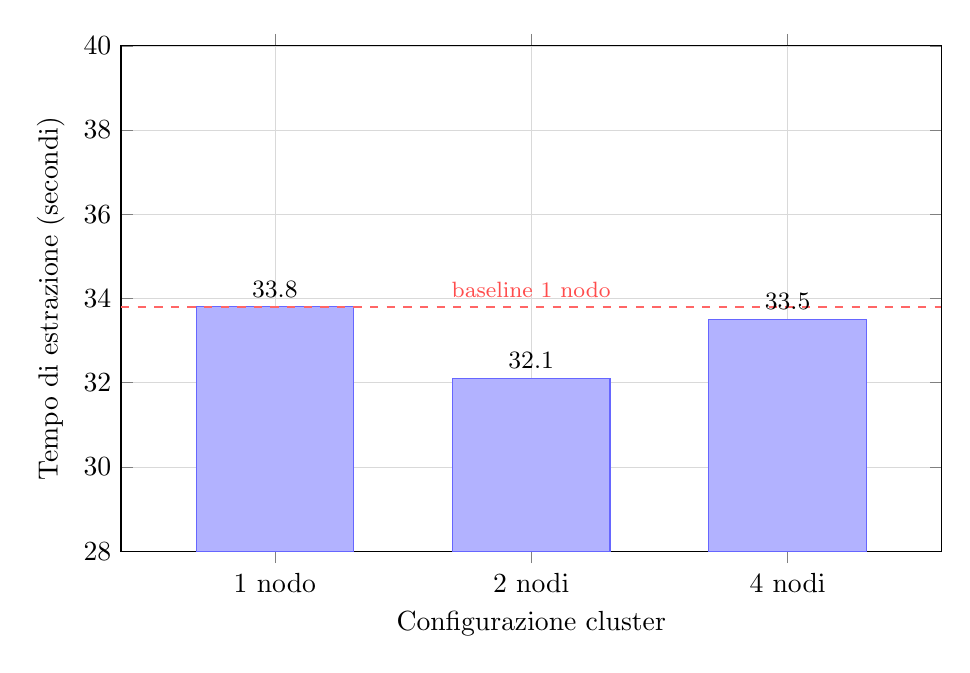
\begin{tikzpicture}
\begin{axis}[
  ybar,
  bar width=2cm,
  width=12cm,
  height=8cm,
  xlabel={Configurazione cluster},
  ylabel={Tempo di estrazione (secondi)},
  symbolic x coords={1 nodo, 2 nodi, 4 nodi},
  xtick=data,
  ymin=28, ymax=40,
  ytick={28,30,32,34,36,38,40},
  nodes near coords,
  nodes near coords align={vertical},
  every node near coord/.style={font=\small, anchor=south},
  enlarge x limits=0.3,
  grid=major,
  grid style={line width=0.2pt, draw=gray!30},
]
\addplot[fill=blue!30, draw=blue!60]
  coordinates {(1 nodo, 33.8) (2 nodi, 32.1) (4 nodi, 33.5)};

% Riga che attraversa tutto il grafico
\draw[dashed, red!60, thick]
  ({rel axis cs:0,0} |- {axis cs:1 nodo, 33.8}) -- ({rel axis cs:1,0} |- {axis cs:1 nodo, 33.8});

% Scritta "baseline 1 nodo" posizionata sopra la linea in corrispondenza del secondo nodo
\node[red!70, font=\footnotesize, above] 
  at (axis cs:2 nodi, 33.8) {baseline 1 nodo};

\end{axis}
\end{tikzpicture}
\caption{Tempi di estrazione nelle tre configurazioni del cluster. La linea tratteggiata evidenzia il baseline a 1 nodo.}
\label{fig:benchmark_bar}
\end{figure}

\subsection{Analisi dei risultati infrastrutturali}

I tempi risultano sostanzialmente costanti tra le tre configurazioni, con una variazione massima di circa 1.7 secondi. Questo risultato, che potrebbe sembrare deludente, è in realtà coerente con la natura del carico di lavoro e con i principi fondamentali dei sistemi distribuiti.

Il bottleneck non è la disponibilità di nodi computazionali, ma la \textbf{capacità di I/O della singola query sequenziale} su un dataset da circa 50 GB. Le tre query Cypher vengono eseguite una dopo l'altra: non esiste parallelismo a livello applicativo che possa sfruttare la presenza di più nodi. Il router Neo4j distribuisce le letture sulle secondary tramite la routing table, ma con una sola connessione attiva alla volta il vantaggio è marginale e viene parzialmente annullato dall'overhead di coordinazione del cluster.

Un dato interessante emerge dal confronto tra le configurazioni a 2 e 4 nodi: la configurazione a 2 nodi risulta leggermente più veloce della configurazione a 4 nodi, come evidenziato nella tabella \ref{tab:benchmark_delta}. 

Questo comportamento suggerisce l'esistenza di un \textit{sweet spot} architetturale: con 2 nodi il bilanciamento tra parallelismo di lettura e overhead di routing è ottimale, mentre l'aggiunta di ulteriori secondary introduce latenze di coordinazione che superano il vantaggio.

Va sottolineato che questo risultato non inficia il valore del cluster. Neo4j Enterprise in configurazione distribuita offre vantaggi significativi che questo benchmark non misura direttamente:

\begin{itemize}
  \item \textbf{Fault tolerance}: con la topologia 1 primary e 3 secondary, il servizio rimane operativo anche in caso di guasto di un nodo, senza interruzione delle letture.
  \item \textbf{Disponibilità}: il routing automatico garantisce la continuità delle operazioni anche durante manutenzioni programmate.
  \item \textbf{Scalabilità su carichi paralleli}: con più client che eseguono query simultanee, il cluster distribuisce il carico sulle secondary producendo speedup significativi, uno scenario non testato in questa tesi ma teoricamente più favorevole.
\end{itemize}


\section{Risultati della Link Prediction}

\subsection{Metriche per modello}

Il training è stato eseguito per \textbf{200 epoche} su \textbf{5 run indipendenti}. Le 200 epoche sono state selezionate per garantire la convergenza di tutti i modelli, verificata monitorando l'andamento della loss. Ciascun modello è stato valutato sul 10\% degli archi tenuti nascosti durante il training tramite \texttt{RandomLinkSplit}, un bilanciamento tra capacità di generalizzazione e dati disponibili sufficienti per una valutazione statisticamente significativa. L'uso di run indipendenti con semi diversi consente di verificare che le differenze prestazionali tra i modelli non siano artefatti dell'inizializzazione casuale dei pesi o della generazione dei campioni negativi.

\begin{table}[ht!]
\centering
\small
\begin{tabular}{lcccc}
\toprule
\textbf{Modello} & \textbf{AUC-ROC medio} & \textbf{Std} & \textbf{Tempo medio (s)} & \textbf{Std (s)} \\
\midrule
GraphSAGE & 0.9934 & 0.0003 & 448.7 & 48.2 \\
HashGNN   & 0.9923 & 0.0002 & 624.2 & 62.1 \\
TransE    & 0.9839 & 0.0006 & 145.2 & 11.8 \\
\bottomrule
\end{tabular}
\caption{Risultati della link prediction Chemical$\to$Disease su 5 run indipendenti, 200 epoche.}
\label{tab:ml_results}
\end{table}

\begin{table}[ht!]
\centering
\small
\begin{tabular}{ccccccc}
\toprule
& \multicolumn{2}{c}{\textbf{GraphSAGE}} & \multicolumn{2}{c}{\textbf{TransE}} & \multicolumn{2}{c}{\textbf{HashGNN}} \\
\cmidrule(lr){2-3} \cmidrule(lr){4-5} \cmidrule(lr){6-7}
\textbf{Run} & \textbf{AUC-ROC} & \textbf{Tempo (s)} & \textbf{AUC-ROC} & \textbf{Tempo (s)} & \textbf{AUC-ROC} & \textbf{Tempo (s)} \\
\midrule
1 & 0.9929 & 471.8 & 0.9839 & 150.6 & 0.9924 & 629.7 \\
2 & 0.9935 & 435.2 & 0.9841 & 144.3 & 0.9926 & 612.5 \\
3 & 0.9938 & 436.5 & 0.9834 & 146.5 & 0.9923 & 623.1 \\
4 & 0.9933 & 454.3 & 0.9838 & 145.8 & 0.9920 & 625.8 \\
5 & 0.9934 & 445.5 & 0.9841 & 143.0 & 0.9924 & 630.1 \\
\bottomrule
\end{tabular}
\caption{Risultati dettagliati per singola run, raggruppati per modello.}
\label{tab:ml_results_detail}
\end{table}

\subsection{Confronto grafico}

\begin{figure}[ht!]
\centering
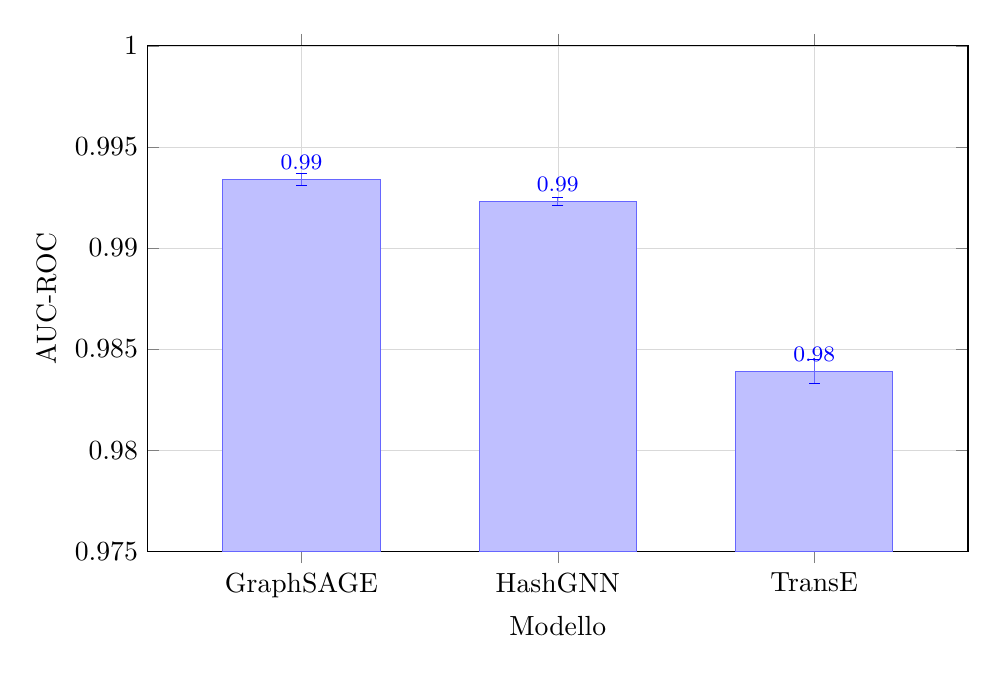
\begin{tikzpicture}
\begin{axis}[
  ybar,
  bar width=2cm,
  width=12cm,
  height=8cm,
  xlabel={Modello},
  ylabel={AUC-ROC},
  symbolic x coords={GraphSAGE, HashGNN, TransE},
  xtick=data,
  ymin=0.975, ymax=1.0,
  ytick={0.975, 0.980, 0.985, 0.990, 0.995, 1.0},
  yticklabel style={/pgf/number format/fixed, /pgf/number format/precision=3},
  enlarge x limits=0.3,
  grid=major,
  grid style={line width=0.2pt, draw=gray!30},
  error bars/y dir=both,
  error bars/y explicit,
  every node near coord/.style={font=\footnotesize, anchor=south},
  nodes near coords,
]
\addplot+[
  fill=blue!25, draw=blue!60,
  error bars/.cd, y dir=both, y explicit
] coordinates {
  (GraphSAGE, 0.9934) +- (0, 0.0003)
  (HashGNN,   0.9923) +- (0, 0.0002)
  (TransE,    0.9839) +- (0, 0.0006)
};
\end{axis}
\end{tikzpicture}
\caption{AUC-ROC medio con deviazione standard per i tre modelli su 5 run indipendenti. L'asse Y parte da 0.975 per rendere visibili le differenze tra i modelli.}
\label{fig:auc_comparison}
\end{figure}

\begin{figure}[ht!]
\centering
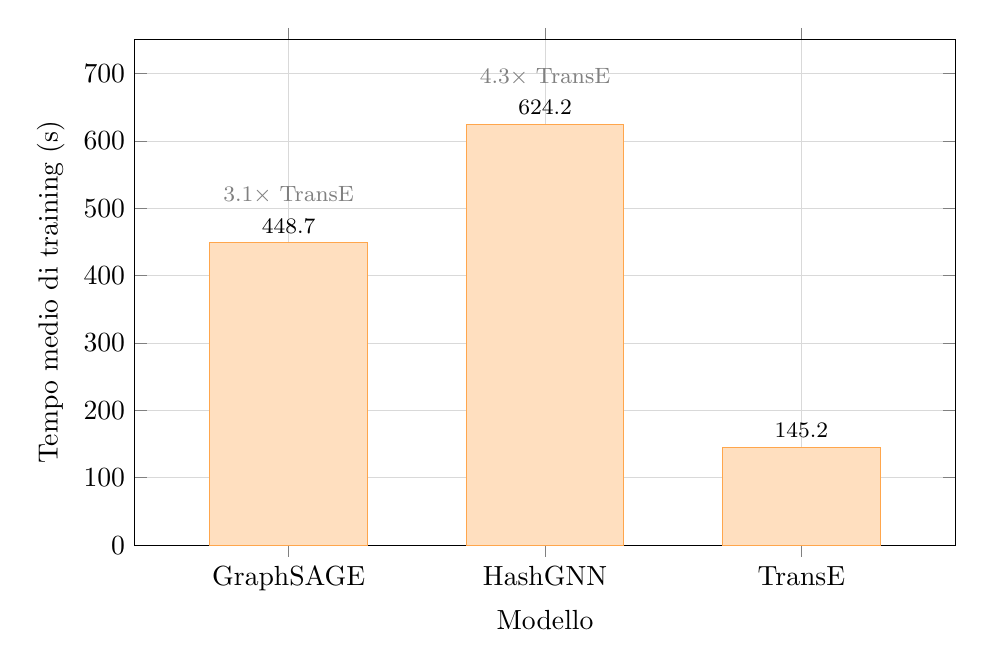
\begin{tikzpicture}
\begin{axis}[
  ybar,
  bar width=2cm,
  width=12cm,
  height=8cm,
  xlabel={Modello},
  ylabel={Tempo medio di training (s)},
  symbolic x coords={GraphSAGE, HashGNN, TransE},
  xtick=data,
  ymin=0, ymax=750,
  ytick={0,100,200,300,400,500,600,700},
  enlarge x limits=0.3,
  grid=major,
  grid style={line width=0.2pt, draw=gray!30},
  nodes near coords,
  every node near coord/.style={font=\footnotesize, anchor=south},
]
\addplot[fill=orange!25, draw=orange!70]
  coordinates {
    (GraphSAGE, 448.7)
    (HashGNN,   624.2)
    (TransE,    145.2)
  };
\node[font=\footnotesize, gray] at (axis cs:GraphSAGE, 520) {\footnotesize $3.1\times$ TransE};
\node[font=\footnotesize, gray] at (axis cs:HashGNN, 695) {\footnotesize $4.3\times$ TransE};
\end{axis}
\end{tikzpicture}
\caption{Tempo medio di training per i tre modelli su 5 run indipendenti}
\label{fig:time_comparison}
\end{figure}


\section{Discussione}

\subsection{Analisi delle prestazioni di GraphSAGE}

GraphSAGE ha registrato l'accuratezza maggiore, con un AUC-ROC medio pari a \textbf{0.9934} e una deviazione standard di 0.0003, denotando un'elevata stabilità statistica nelle diverse esecuzioni. Tale evidenza empirica diverge dall'ipotesi preliminare, che postulava una superiorità di HashGNN in virtù della sua gestione nativa dell'eterogeneità.

Le prestazioni ottimali di GraphSAGE possono essere ricondotte a due fattori. Il primo risiede nella \textbf{fusione degli spazi di embedding}: concatenando le rappresentazioni dei due tipi di nodo in unico spazio latente con \textit{offset}, il modello induce le entità a condividere le stesse coordinate geometriche sin dalle fasi iniziali dell'addestramento. Questa convergenza spaziale riduce la complessità a carico \textit{decoder} MLP nell'inferire la probabilità di collegamento. Il secondo fattore riguarda la \textbf{velocità di convergenza}: le matrici dei pesi nei layer SAGEConv, dense ottimizzabili gradiente, garantiscono una propagazione del segnale efficiente rispetto alle architetture basate su proiezioni fisse.

Nonostante i risultati ottenuti, occorre ribadire un limite teorico di GraphSAGE già evidenziato in sede di analisi esplorativa: il modello aggrega i dati del vicinato in modo omogeneo, non distinguendo la tipologia semantica delle relazioni. Sebbene all'interno del sottografo isolato (Chemical$\to$Disease) ciò non costituisca un fattore penalizzante, poiché tutte le relazioni condividono il medesimo significato semantico, l'applicazione su un grafo eterogeneo completo comporterebbe verosimilmente un degrado fisiologico delle prestazioni predittive.

\subsection{Analisi delle prestazioni di HashGNN}

HashGNN si posiziona immediatamente al di sotto di GraphSAGE con un AUC-ROC medio di \textbf{0.9923} (scarto di 0.0011). Considerando la deviazione standard (0.0002), le distribuzioni dei risultati dei due modelli risultano statisticamente sovrapponibili in gran parte: in un contesto applicativo legato al \textit{drug repurposing}, tale differenza di accuratezza risulta trascurabile ai fini operativi.

Tuttavia, si osserva una marcata disparità in termini di \textbf{complessità temporale}: con un valore medio di 624 secondi per 200 epoche, l'addestramento di HashGNN risulta circa 1.4 volte più oneroso rispetto a GraphSAGE e 4.3 volte superiore rispetto a TransE. Questo incremento è imputabile all'uso delle proiezioni \textit{hash} fisse. I layer lineari successivi richiedono un maggior numero di iterazioni per processare rappresentazioni binarizzate e stocastiche. Poiché le matrici di \textit{hashing} non sono soggette ad aggiornamento via \textit{backpropagation}, l'ottimizzazione grava interamente sui layer lineari dedicati, i quali devono compensare l'iniziale trasformazione aleatoria, rallentando di conseguenza la convergenza.

L'aspettativa teorica di una predominanza di HashGNN non ha trovato riscontro empirico nel perimetro sperimentale analizzato. L'assenza di un vantaggio misurabile suggerisce che, per questo specifico dominio relazionale, l'omofilia biologica intrinseca al sottografo è sufficientemente delineata da poter essere appresa in modo ottimale da un modello omogeneo, rendendo superflua una gestione esplicita dell'eterogeneità.

\subsection{Analisi delle prestazioni di TransE}

TransE ha conseguito un AUC-ROC medio pari a \textbf{0.9839}, posizionandosi al di sotto di GraphSAGE di circa un punto percentuale, ma con un tempo di addestramento significativamente ridotto, pari a soli \textbf{145 secondi}. Ciò qualifica l'algoritmo come la soluzione computazionalmente più efficiente tra quelle in esame, con un rapporto costo-prestazioni che lo rende particolarmente interessante per scenari operativi con risorse limitate, dove la riduzione dei tempi di calcolo può tradursi in minori costi infrastrutturali e maggiore flessibilità operativa. Tale efficienza è il risultato diretto di un'architettura essenziale: il modello non implementa meccanismi di \textit{message passing} né layer convoluzionali per l'aggregazione del vicinato. L'aggiornamento dei pesi si basa esclusivamente su operazioni di \textit{lookup} all'interno delle matrici di embedding e sul calcolo della distanza L2, calcoli caratterizzati da una bassa complessità asintotica e da un'elevata scalabilità anche su topologie di grandi dimensioni. A differenza delle GNN, che richiedono la propagazione del segnale attraverso l'intero vicinato, TransE opera indipendentemente dalla densità locale del grafo, mantenendo costante il costo per epoca di training, un vantaggio non trascurabile quando si lavora con grafi che presentano nodi con grado estremamente elevato.

È fondamentale osservare che, nel contesto di questo studio, TransE non ha potuto sfruttare appieno la sua capacità di codificare esplicitamente relazioni semanticamente distinte (attraverso l'ottimizzazione del vettore di traslazione $\mathbf{r}$), in quanto gli archi all'interno del sottografo sono stati trattati come appartenenti a un'unica classe relazionale. In un'analisi estesa all'intera topologia multimodale di PharMeBiNet, tale modello potrebbe far emergere in modo più netto i propri vantaggi teorici rispetto agli approcci convoluzionali standard, dove la distinzione semantica delle relazioni viene invece appiattita dall'aggregazione omogenea del vicinato, confermando come la scelta dell'algoritmo debba essere guidata dalla complessità semantica del grafo e dalle priorità operative del contesto applicativo.

\subsection{Analisi del trade-off tra accuratezza ed efficienza}
La Figura \ref{fig:tradeoff} illustra la distribuzione dei modelli nello spazio dimensionale definito da accuratezza ed efficienza computazionale. L'analisi grafica evidenzia una condizione rilevante: \textbf{GraphSAGE domina HashGNN in senso di Pareto}. A parità di fascia di accuratezza, GraphSAGE raggiunge la convergenza in un tempo strettamente inferiore; di conseguenza, all'interno dei confini di questo studio, l'adozione di HashGNN non trova una giustificazione operativa oggettiva rispetto alla controparte. Questo risultato suggerisce che la complessità aggiuntiva introdotta dalla gestione separata degli spazi di embedding non si traduce in un vantaggio predittivo misurabile sul sottografo considerato, probabilmente perché la relazione Chemical-Disease presenta un'omofilia strutturale sufficientemente forte da essere catturata efficacemente da un modello omogeneo senza la necessità di spazi di rappresentazione distinti.

TransE, al contrario, si colloca in un distinto quadrante dello spazio delle soluzioni, configurandosi come un'alternativa operativa indipendente. In contesti industriali caratterizzati da volumi di dati su larga scala o da necessità di riaddestramento frequente, l'accettazione di una lieve flessione nell'accuratezza (circa 0.01 in termini di AUC) costituisce un compromesso metodologico razionale a fronte di un abbattimento dei tempi di esecuzione nell'ordine del 67\%. Questo trade-off assume particolare rilevanza in scenari di produzione dove i modelli devono essere aggiornati periodicamente su nuovi dati, rendendo il costo computazionale un fattore critico almeno quanto l'accuratezza predittiva, soprattutto quando le risorse di calcolo sono limitate o i vincoli temporali impongono risposte rapide.

\begin{figure}[ht!]
\centering
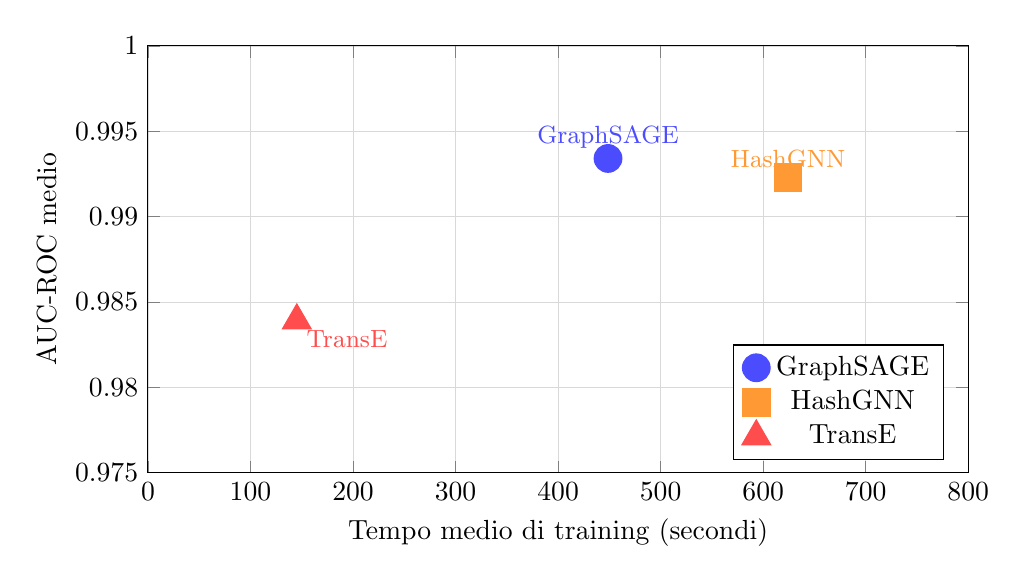
\begin{tikzpicture}
\begin{axis}[
  width=12cm,
  height=7cm,
  xlabel={Tempo medio di training (secondi)},
  ylabel={AUC-ROC medio},
  xmin=0, xmax=800,
  ymin=0.975, ymax=1.0,
  yticklabel style={/pgf/number format/fixed, /pgf/number format/precision=3},
  grid=both,
  grid style={line width=0.2pt, draw=gray!30},
  legend pos=south east,
]
\addplot[only marks, mark=*, mark size=5pt, blue!70] coordinates {(448.7, 0.9934)};
\addlegendentry{GraphSAGE}
\addplot[only marks, mark=square*, mark size=5pt, orange!80] coordinates {(624.2, 0.9923)};
\addlegendentry{HashGNN}
\addplot[only marks, mark=triangle*, mark size=6pt, red!70] coordinates {(145.2, 0.9839)};
\addlegendentry{TransE}
\node[blue!70, font=\small, anchor=south] at (axis cs:448.7, 0.9934) {GraphSAGE};
\node[orange!80, font=\small, anchor=south] at (axis cs:624.2, 0.9923) {HashGNN};
\node[red!70, font=\small, anchor=north west] at (axis cs:145.2, 0.9839) {TransE};
\end{axis}
\end{tikzpicture}
\caption{Trade-off tra accuratezza ed efficienza computazionale per i tre modelli.}
\label{fig:tradeoff}
\end{figure}



\subsection{Verifica delle ipotesi sperimentali}

L'impianto teorico preliminare postulava un ordinamento decrescente delle prestazioni dominato da HashGNN, seguito da TransE e infine da GraphSAGE. L'evidenza empirica ha restituito una gerarchia differente: GraphSAGE ha mostrato i risultati più solidi, seguito a breve distanza da HashGNN e successivamente da TransE.

Dal punto di vista infrastrutturale, l'atteso incremento di \textit{throughput} associato all'impiego di un cluster distribuito a 4 nodi rispetto a un'istanza singola non ha trovato conferma. Tale risultato, pienamente coerente con i paradigmi teorici dei sistemi distribuiti per operazioni di I/O, dimostra empiricamente che, in presenza di flussi di estrazione dati sequenziali di tipo \textit{batch}, la scalabilità orizzontale di Neo4j non comporta riduzioni dei tempi di latenza. Il reale beneficio dell'architettura distribuita risiede pertanto nell'alta disponibilità e nella tolleranza ai guasti (\textit{fault tolerance}), non nell'accelerazione intrinseca della singola interrogazione sequenziale.

L'analisi degli scostamenti tra le aspettative teoriche e i riscontri empirici fornisce un elemento di valutazione centrale: attesta che i vantaggi offerti da architetture software o algoritmiche sofisticate necessitano di specifiche condizioni al contorno per potersi manifestare, come la presenza di un grafo nativamente eterogeneo per HashGNN o l'esecuzione di carichi interrogativi fortemente paralleli nel caso del cluster distribuito.